% Appendix A

% variables
\newcommand{\appdira}{appendices/plots/appendixA}

\chapter{Dark matter formulas and calculations} % Main appendix title

\label{AppendixA} % For referencing this appendix elsewhere, use \ref{AppendixA}

%\section{Thermal Dark Matter}
%\label{appA:sec:thermal-dark-matter}

\section{Calculation of $\ae$ cross-section using the Weizsacker-Williams approximation}
\label{appA:sec:cross-section-wz}

In this section, we calculate the cross-section of the Dark Bremsstrahlung process used by NA64 for the signal yield:

\begin{equation}
  \label{eq:dp-cs}
  \frac{d\sigma(e(p) + Z(P_i) \to e(p') + Z(P_f) + A'(k))}{dE_{\DM}d\cos{\theta_{\DM}}}
\end{equation}

Following the method in \cite{jdb}. We use the WW approximation, where $k=(E_{\DM},\vec{k})$ is the momentum of the emitted Dark Photon and $\theta_{\DM}$ is the angle relative to the incoming momentum of the electron $p$ in the lab frame. In the scenario of a fixed target experiment, we set the target at rest $P_i = (M,0)$ and the primary to the nominal beam energy $p = (E_0, \vec{p})$.

In the WW approximation picture, in the frame of the electron we see rapidly moving atom sources emitting a cloud of effective photons that the primary electron irradiates with to emit an $\DM$. This means we can reduce the cross section to the one of a real photon scattering, i.e. $e(p) + \gamma(q) \to e(p') + A(k)$ where the photon transports the difference of energy between initial and final state of the nucleus $q = P_f - P_i$. In this picture we redefine Eq.\ref{eq:dp-cs}:

\begin{equation}
  \label{eq:dp-cs-ww}
  \begin{aligned}
    \frac{d\sigma(e(p) + Z(P_i) \to e(p') + Z(P_f) + A'(k))}{dE_{\DM}d\cos{\theta_{\DM}}} = &\left(\frac{\alpha \chi}{\pi} \right) \left(\frac{E_0 x \beta_{\DM}}{(1 - x)} \right) \\
    &\times \left( \frac{d\sigma(e(p) + \gamma(q) \to e(p') + \DM(k))}{d(p \cdot k)} \right)_{t = t_{min}}
   \end{aligned}
 \end{equation}

 Where $x=E_{\DM}/E_0$ is the fraction of energy transfer to $\DM$ and $t=-q^2$. For a given four-momentum $k$ the virtuality $t$ has a minimum value $t_{min}$ when $\vec{q}$ is collinear with the vector $(\vec{k} - \vec{p})$. In this collinear geometry, we can solve the mass shell condition $(q + p - k)^2 = m^2_e$ and $P^2_f = (P_i - q)^2$:

 \begin{equation}
   \label{eq:t-min}
   t_{min} = -q^2_{min} \approx \left(\frac{\rm{U}}{2E_0 (1 - x)} \right)
 \end{equation}

 Where we define $\rm{U}$ using only leading effects:

 \begin{equation}
   \label{eq:dp-u}
   \rm{U}(x, \theta_{\DM}) = E_0^2 \theta_{\DM}x + m^2_{\DM} \frac{1-x}{x} + m^2_e x
 \end{equation}

 Using this kinematics, we can express the following variables:

 \begin{equation}
   \label{eq:dp-md-var}
   \begin{aligned}
     &-\widetilde{u} \equiv m_e^2 - u_2 = 2p\cdot k - m^2_{\DM} = \rm{U}\\
     &\widetilde{s}  \equiv s_2 - m_e^2 = 2p' \cdot k + m^2_{\DM} = \frac{\rm{U}}{1-x} \\
     &t_2 = (p - p')^2 = - \frac{\rm{U}x}{1-x} + m^2_{\DM}
   \end{aligned}
 \end{equation}

 where $s_2$, $u_2$ and $t_2$ are the Mandelstam variables of the process. We compute the cross section as function of the variable defined above \cite{jdb}:

 \begin{equation}
   \label{eq:dp-cs-comp}
   \begin{aligned}
     \frac{d \sigma}{d(p \cdot k)} = 2 \frac{d\sigma}{dt_2} &\approx \frac{1}{8 \pi (s_2 - m^2_e)} |M|^2 \\
     &=\frac{4 \pi \alpha^2 \epsilon^2}{\widetilde{s}^2} \left( \frac{\widetilde{s}}{-\widetilde{u}} + \frac{-\widetilde{u}}{\widetilde{s}} + \frac{s m^2_{\DM} t_2}{-\widetilde{u}\widetilde{s}} \right) \\
           &=\underline{(4 \pi \alpha^2 \epsilon^2) \frac{(1-x)}{\rm{U}^2} \left[ 1 + (1 - x)^2 + \frac{2(1-x)^2m^2_{\DM}}{\rm{U}^2} \left( m^2_{\DM} - \frac{\rm{U}x}{1-x} \right) \right]}
   \end{aligned}
 \end{equation}

 In the last step, the equation was expanded in the order $m^2_e$.

 Now that we calculated the cross section of the $2 \to 2$ process we can plug it in Eq.\ref{eq:dp-cs-ww} to reach a complete formula of the WW cross-section:

 \begin{equation}
   \label{eq:dp-cs-ww-num}
   \frac{1}{E^2_0} \frac{d\sigma_{WW}}{dx d\cos{\theta_{\DM}}} = (8 \alpha^3 \epsilon^2 \chi \beta_{\DM}) \left[ \frac{1 - x + x/2}{\rm{U}^2} + \frac{(1-x)^2m^2_{\DM}}{\rm{U}^4} \left(m^2_{\DM} - \frac{\rm{U}x}{1 - x} \right) \right]
 \end{equation}

 To obtain a differential cross-section for $dx$ we need to integrate the equation above for $\cos{\theta_{\DM}}$. There are two problems to this integral:

 \begin{itemize}
 \item In the limit $m^2_{\DM} \to 0$ the denominator $\rm{U}(x, \theta_{\DM} = 0)$ becomes singular in $x \to 0$, which is the standard Bremsstrahlung singularity of photons.   
 \item The term $\chi$ can depend on $\theta_{\DM}$.
 \end{itemize}

 The singularity is in most of the cases of interest regulated by the Dark Photon mass. For the case $m_{\DM} \gg m_e$ the denominator takes the form $\rm{U} \approx m^2_{\DM} \frac{1-x}{x}$.
 $\chi$ on the other hand is an effective flux of photons that is integrated from the minimum to maximum momentum exchange $t_{min}$/$t_{max}$. For a general electric form factor $G_2(t)$:

 \begin{equation}
   \label{eq:g-ff}
   \chi = \int^{t_{max}}_{t_{min}} dt \frac{t - t_{min}}{t^2} G_2(t)
 \end{equation}

 The form factor $G_1(t)$ is relevant only for a negligible amount of the case of interest and is here neglected. As discussed in \cite{Kim:1973he,RevModPhys.46.815}, the maximum momentum transfer can be set to be $t_{max} \sim m^2_{\DM}$, where the matrix element of $2 \to 3$ drops dramatically. We divide the form factor in elastic and inelastic component \cite{jdb}:

 \begin{align}
   \label{eq:g-ff-el}
   &G_{2,el}(t) = \left( \frac{a^2 t}{1 + a^2t} \right)^2 \left( \frac{1}{1 + t/d}\right) Z^2\\
   \label{eq:g-ff-in}
   &G_{2,in}(t) = \left( \frac{a'^2 t }{1 + a'^2 t} \right)^2 \left( \frac{1 + t (\mu_p^2 -1) / (4m^2_p)}{(1 + t / (\SI{0.71}{\giga\electronvolt\squared})^4} \right) Z
 \end{align}

 The parametrization becomes uncertain for high masses of the Dark Photon, but they are reliable for the ranges of interest in NA64 of $m^2_{\DM} < \SI{1}{\giga\electronvolt}$. Numerically, the factor $\chi / Z^2$ depends on the beam energy used, but can be set to be $\chi/Z^2 \mathcal{L}og \approx 5-10$ for the NA64 case. As we can see, we can neglect in good approximation the angular dependence of $\chi$ using these formulas. Coming back at Eq.\ref{eq:dp-cs-ww-num}, we drop $m^2_e$ and perform the integration on the angle and obtain a form for the $dx$ differential cross-section. The results is Eq.\ref{eq:dm-diff-cross} that we reported in chapter \ref{chapter1}, with the flux of photon $\chi$ expressed as the constant $\mathcal{L}og$:

 \begin{equation}
   \label{eq:dp-cs-dx}
\frac{d\sigma_{WW}}{dx} \approx \frac{8 Z^2 \alpha^3 \epsilon^2 x}{m^2_{\DM}} \left( 1 + \frac{x^2}{3(1-x)} \right) \mathcal{L}og    
\end{equation}


\subsection{Production rate}
\label{appA:sec:production-rate}

TO compute the production rate, we integrated the differential cross section compute above in the scenario of an high-energy electron impacting a fixed-target of $T$ radiation lengths used in chapter \ref{chapter1}:


\begin{equation}
  \label{eq:dm-gy}
  \frac{dN}{dx} = N_e \frac{N_0 X_0}{A} \int_{E_{\DM}}^{E_0} \frac{dE_1}{E_1} \int_0^T dt I(E_1;E_0;t) \times E_0 \frac{d\sigma}{dx'}\Big|_{x' = E_{\DM}/E_1}
\end{equation}

We need first to parametrize the energy distribution of the electrons after $t$ radiation lengths. Here we assume the production of $\DM$ will happen in the first few radiation length, hence we neglect the $t$ dependence, and we use the paramterization \cite{jdb}:

\begin{equation}
  \label{eq:i-dist}
  I(E_1;E_0,t) \approx  \frac{1}{E_0} y^{bt-1} bt \quad T \gtrsim 1
\end{equation}

where we take $y = \frac{E_) - E_1}{E_0}$ and $b=4/3$. With this we find:

\begin{equation}
  \label{eq:i-int}
  \widetilde{I} = \int^T_0 dt I(E_1; E_0, t) \approx \frac{1 + y^{bT}(bT\ln{y} - 1}{E_0by(\ln{y})^2} \underbrace{\to}_{T \to \infty} \frac{1}{E_0by(\ln{y})^2}
\end{equation}

Where the last approximation is correct within 1\% for $T>7$ and $0.5 < y$. This equation account for the constant $C'$ that multiples the signal rate in Eq.\ref{eq:dm-rate}. We stress that although the scaling is well reproduced using this method, the numerical result produced still has a significant uncertainty that depends on the exact scenario considered. For a precise computation of the signal yield, the exact tree-level cross-section is used instead, implemented inside an MC simulation to reproduce the em-shower and the efficiency of the cuts.



\section{The Tree-level corrections}
\label{appA:sec:cross-section-tl}

In the NA64 experiment, the cross section is compute using precise tree-level calculation instead of one based on the IWW approximation \cite{DMsimulation}. We start again using the notation of momenta used in Eq.\ref{eq:dp-cs}, and we perform the calculations in the frame of reference where the vector $\bf{V} = \bf{p} - \bf{k}$ is parallel to the z-axis and the vector $\bf{k}$ is in the xz-plane. We can express the relevant cross-section using the formula:

\begin{equation}
  \label{eq:cs-tl}
  \frac{d\sigma}{dx d\cos{\theta}} = \frac{\epsilon^2 \alpha^3 |\bf{k}| E_0}{|\bf{p}| |\bf{k} - \bf{p}|} \cdot \int_{t_{min}}^{t_{max}} \frac{dt}{t^2} g^{el}_{2}(t) \cdot \int_0^{2\pi} \frac{d\phi_q}{2\pi} \frac{|A^{2 \to 3}_{\DM}|^22}{8 M^2}
\end{equation}

Where the angle $\phi_q$ is the axial angle of $\bf{q}$ defined in Eq.\ref{eq:t-min}. and $|A^{2 \to 3}_{\DM}|$ is the matrix element of the Dark Bremsstrahlung. We define the boundary of the first integral as in the previous section, and we express the amplitude squared of the cross section as:

\begin{equation}
  \label{eq:cs-dp-amp}
  \begin{aligned}
    |A^{2 \to 3}_{\DM}|^2 = \frac{2}{\widetilde{s}^2\widetilde{t}^2} \Big( &2m^2_e (\mathcal{P}^2 t (\widetilde{s} + \widetilde{u})^2 - 4((\mathcal{P} \cdot p)\widetilde{u} + (\mathcal{P} \cdot p')\widetilde{s})^2  \\
      &+ m^2_{\DM}(\mathcal{P}^2 t (\widetilde{s} - \widetilde{u})^2 -4((\mathcal{P}\cdot p)\widetilde{u} + (\mathcal{P}\cdot p')\widetilde{s})^2 \\
      &+ \widetilde{s}\widetilde{u}(\mathcal{P}^2 ((\widetilde{s} + t)^2 + (\widetilde{u}+t)^2) - 4 t ((\mathcal{P} \cdot p)^2 + (\mathcal{P} \cdot p')^2) \Big)
  \end{aligned}    
\end{equation}

Where we used the Mandelstam variables defined in Eq.\ref{eq:dp-md-var} (without the last equivalence to $\rm{U}$) and:

\begin{equation}
  \label{eq:dp-md-var-2}
  \mathcal{P}^2 = 4M^2 + t, \quad \mathcal{P} \cdot p = 2 M E_0 k_0 - (\widetilde{s} + t)/2, \quad \mathcal{P} \cdot p' = 2 M (E_0 - k_0) + (\widetilde{u} - t)/2
\end{equation}

Next we perform the integration over $\phi_q$ to find \cite{DMsimulation}:

\begin{equation}
  \label{eq:dp-cs-tl-int}
  \int_0^{2\pi} \frac{d\phi_q}{2\pi} |A^{2 \to 3}_{\DM}|^2 = A^{(0)}_{\DM} + Y \cdot A^{(1)}_{\DM} + \frac{1}{W^{1/2}} \cdot A^{(-1)}_{\DM} + \frac{Y}{W^{2/3}} \cdot A^{(-2)}_{\DM}
\end{equation}

Where we divided the calculation of the cross-section as the sum of different amplitudes:

\begin{equation}
  \label{eq:dp-cs-tl-par}
  \begin{aligned}
    &A^{(-2)}_{\DM} = -8M (4E_0M - t(2E_0 + M ))(m^2_{\DM} + 2m^2_e)\\
    &A^{(-1)}_{\DM} = \frac{8}{\widetilde{u}} \Big[ M^2 (2t\widetilde{u} + \widetilde{u}^2 + 4E_0^2 (2(x-1)(m^2_{\DM} + 2m_e^2) - t((x-2)x + 2)\\
    &+ 2t(-m^2_{\DM} - 2m_e^2 + t)) - 2E_0 M t ((1-x)\widetilde{u} + (x-2)(m^2_{\DM} + 2m^2_e + t) + t^2 (\widetilde{u} - m^2_{\DM}) \Big] \\
    &A^{(0)}_{\DM} = \frac{8}{\widetilde{u}^2} \Big[ M^2 (2t\widetilde{u} + (t - 4E_0^2(x-1)^2)(m^2_{\DM} + 2m^2_e)) + 2E_0M t (\widetilde{u} - (x-1)(m^2_{\DM} + 2m^2_e)) \Big] \\
    &A^{(1)}_{\DM} = \frac{8M^2}{\widetilde{u}} \\
    &Y = q^2 + 2q_0 E_0 - 2 \frac{|\bf{q}| |\bf{p}|}{\bf{p} - \bf{k}|} (|\bf{p} - \bf{k} \cos{\theta})\cos{\theta_q}, \quad W = Y^2 - 4 \frac{|\bf{q}|^2|\bf{p}|^2|\bf{k}|^2}{|\bf{q} - \bf{k}|^2} \sin{\theta}^2\sin{\theta_q}^2
  \end{aligned}
\end{equation}

To derive the total cross-section it is needed the numerical computation of Eq.\ref{eq:cs-tl} along with all allowed range of $x$ and $\theta$ (which is shown as an explicit $t$ integration in the equation). For a benchmark calculation the invisible mode scenario was used, using Lead as target ($Z = 82$) and $E_0 = 100 \gev$. Fig.\ref{fig:dp-cs-tl} show the results of these calculation as the differential cross-section calculate for different mass as function of $x$. The classical Bremsstrahlung of gamma is also shown as implemented in Geant4 which agrees remarkably with the above calculation when a mass $m_{\DM} = 0$ is used, for a total relative disagreement of 8\%. In NA64, the expression used avoids infrared divergencies as the Dark Photon is expected to be massive. Moreover, the large cut used in NA64 searches $E^{ECAL}_{miss} > 50 \gev$ cut the part of the spectrum containing the divergency even for $\DM$ mass close to zero.

\begin{figure}[bth!]
  \centering
  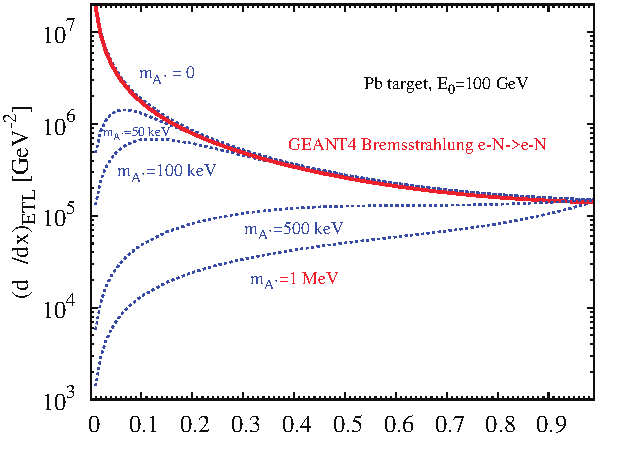
\includegraphics[width=\textwidth]{\appdira/tree-level-na64-calc.pdf}
  \caption[Tree level differential cross-section for different masses]{Differential cross-section of $\DM$ production via Bremsstrahlung as function of $x=E_{\DM}/E_0$ for different masses and $\epsilon = 1$ calculated using tree-level calculations. Red line show the same spectrum used in Geant4 for the standard Bremsstrahlung $e + Z \to e + Z + \gamma$. Target used was lead with a primary energy $E_0 = 100 \gev$ \cite{DMsimulation}}
  \label{fig:dp-cs-tl}
\end{figure}

\subsection{Implementation inside the Geant4 simulation}

To implement the Exact Tree Level (ETL), we define the following ratio (called $K$-factor):

\begin{equation}
  \label{eq:k-factor}
  K(m_{\DM},E_0,Z,A) = \sigma^{\DM}_{IWW} / \sigma^{\DM}_{ETL}
\end{equation}

which is numerically the correction to the cross-section calculated in the IWW approximation. We show the numerical value of this $K$-factor as a function of the primary energy $E_0$ for different masses in Fig.\ref{fig:k-factor}.

\begin{figure}[bth!]
  \centering
  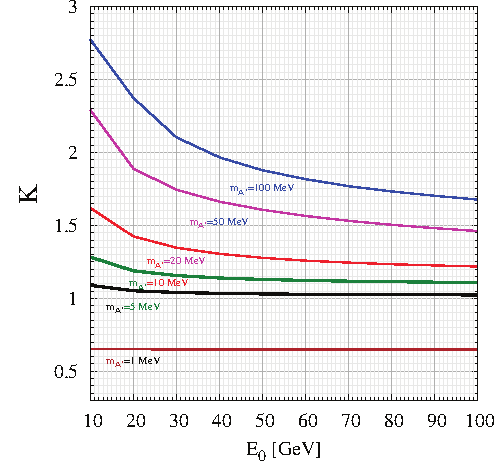
\includegraphics[width=\textwidth]{\appdira/k-factor.pdf}
  \caption{Ratio between cross-section calculated in the IWW approximation and using ETL computation $K = \sigma^{\DM}_{IWW} / \sigma^{\DM}_{ETL}$ described in Sec.\ref{appA:sec:cross-section-tl} for different Dark photon masses.}
  \label{fig:k-factor}
\end{figure}

For the simulation, the $K$-factors are tabulated and used to extract the real cross-section for a general case. The cross-section is calculated precisely for several benchmark cases (the same one shown in Fig.\ref{fig:k-factor}) and then extrapolated using a Bilinear interpolation.

% The color of links can be changed to your liking using:

% {\small\verb!\hypersetup{urlcolor=red}!}, or

% {\small\verb!\hypersetup{citecolor=green}!}, or

% {\small\verb!\hypersetup{allcolor=blue}!}.

% \noindent If you want to completely hide the links, you can use:

% {\small\verb!\hypersetup{allcolors=.}!}, or even better: 

% {\small\verb!\hypersetup{hidelinks}!}.

% \noindent If you want to have obvious links in the PDF but not the printed text, use:

% {\small\verb!\hypersetup{colorlinks=false}!}.

%%% Local Variables:
%%% mode: latex
%%% TeX-master: "../PhDthesis"
%%% End:
